\documentclass[preprint,12pt]{elsarticle}

% ------- Packages -------
\usepackage{graphicx}
\usepackage{amsmath,amssymb}
\usepackage{booktabs,multirow}
\usepackage{siunitx}
\usepackage{caption}
\usepackage{subcaption}
\usepackage{float}
\usepackage{enumitem}
\usepackage{xcolor}
\usepackage{hyperref}
\usepackage[utf8]{inputenc}   

% Captions + hyperlinks
\captionsetup{font=small,labelfont=bf}
\hypersetup{
  colorlinks=true,
  linkcolor=blue!60!black,
  citecolor=blue!60!black,
  urlcolor=blue!60!black
}

% Elsevier natbib options (author–year)
\biboptions{authoryear}

% Where your figures/tables live
\graphicspath{{output/}{figures/}}

\begin{document}
\begin{frontmatter}

\title{Ensemble Deep Learning for Robust Skin Lesion Classification:\\
A Comprehensive Study on HAM10000}

\author[inst1]{Md Naim Hassan Saykat\corref{cor1}}
\cortext[cor1]{Corresponding author: md-naim-hassan.saykat@universite-paris-saclay.fr}
\address[inst1]{Department of Computer Science, Université Paris-Saclay, Orsay, France}

\journal{Expert Systems With Applications}

\begin{abstract}
\textbf{Background:} Skin cancer is one of the most prevalent malignancies worldwide, with melanoma being particularly lethal if not detected early. Automated deep learning methods have shown promise in dermoscopic image classification, yet individual models often lack robustness across heterogeneous lesion types.

\textbf{Methods:} We developed an ensemble of seven deep learning architectures---CNN, ResNet-50, DenseNet-121, EfficientNet-B3, ConvNeXt-Tiny, MobileNetV3, and Vision Transformer (ViT)---trained on the HAM10000 dataset. Predictions were fused via mean probability aggregation, following label alignment across models. Performance was evaluated on a stratified test set using Accuracy, Weighted F1, and ROC--AUC (macro/micro). Uncertainty and statistical robustness were assessed with bootstrap confidence intervals, McNemar’s test, and $\Delta$-metrics. Model calibration was examined via Expected Calibration Error (ECE), and interpretability was explored through Grad-CAM visualizations.

\textbf{Results:} All models achieved strong performance (ROC--AUC $>0.90$), with the ensemble consistently outperforming individual architectures across all metrics. Improvements were statistically significant in most comparisons. Calibration analysis showed competitive reliability, and Grad-CAM highlighted clinically relevant lesion regions.

\textbf{Conclusion:} The proposed ensemble provides a robust, accurate, and interpretable tool for skin lesion classification, reducing variance compared to single backbones. This framework has potential to support dermatologists in early melanoma detection, improve diagnostic reliability, and reduce clinical risk. Future work will extend validation to larger datasets and explore advanced ensembling strategies for clinical deployment.

\textbf{Keywords:} Skin lesion classification; Ensemble learning; Deep learning; HAM10000; Explainable AI; Medical imaging.
\end{abstract}

\end{frontmatter}

% =========================
\section{Introduction}

Skin cancer represents one of the most common and rapidly increasing malignancies worldwide. Among its variants, melanoma accounts for the majority of skin cancer-related deaths due to its aggressive progression and high metastatic potential. Early and accurate diagnosis is therefore essential to improve patient survival and reduce healthcare burden. Dermoscopy has become a standard imaging modality for lesion assessment, yet diagnostic interpretation remains highly operator-dependent and subject to inter-observer variability, even among expert dermatologists \citep{tschandl2018ham10000}.

Deep learning has shown remarkable success in medical image classification, achieving dermatologist-level performance in several studies \citep{esteva2017dermatologist}. Convolutional neural networks (CNNs) and, more recently, Transformer-based architectures have emerged as powerful tools for skin lesion analysis. Despite their success, individual models often struggle with robustness, generalization, and calibration across heterogeneous lesion types, class imbalance, and dataset variability. These limitations restrict their direct clinical adoption.

Ensemble learning offers a potential solution by combining complementary strengths of diverse models to improve accuracy, reduce variance, and enhance reliability \cite{dietterich2000ensemble}. Prior studies in medical imaging have demonstrated that ensembles not only improve predictive performance but also provide more stable and trustworthy outputs \citep{valverde2021ensembles}. However, systematic investigations of ensemble approaches in dermoscopic image classification remain limited, particularly with comprehensive statistical validation and interpretability analyses.

In this work, we address these gaps by developing and evaluating an ensemble of seven deep learning models---CNN, ResNet-50, DenseNet-121, EfficientNet-B3, ConvNeXt-Tiny, MobileNetV3, and Vision Transformer (ViT)---on the HAM10000 dataset \cite{tschandl2018ham10000}. We benchmark individual architectures and their ensemble across Accuracy, Weighted F1, and ROC--AUC metrics, incorporating bootstrap confidence intervals and McNemar’s test to ensure statistical rigor. Furthermore, we evaluate calibration using Expected Calibration Error (ECE) and provide Grad-CAM visualizations to enhance clinical interpretability.

The main contributions of this study are threefold:
\begin{itemize}[leftmargin=1.5em]
    \item We present a diverse ensemble framework that consistently outperforms individual backbones on the HAM10000 dataset, demonstrating significant performance gains validated by statistical testing.
    \item We provide a comprehensive evaluation including confidence intervals, McNemar’s test, $\Delta$-metrics, and calibration analysis, ensuring robust and clinically meaningful comparisons.
    \item We enhance interpretability by generating Grad-CAM visualizations, highlighting clinically relevant lesion regions that align with dermatological reasoning.
\end{itemize}

Through this work, we demonstrate that ensembles not only advance performance but also improve reliability and interpretability, thereby offering a viable pathway toward clinically deployable AI-assisted skin lesion classification systems.

% =========================
\section{Related Work}

\subsection{Deep Learning for Skin Lesion Classification}
The application of deep learning to dermoscopic image analysis has grown substantially over the past decade. Early work by Esteva et al.\ \cite{esteva2017dermatologist} demonstrated dermatologist-level classification performance using convolutional neural networks (CNNs) trained on large-scale skin lesion datasets. Subsequent studies leveraged public benchmarks such as ISIC and HAM10000 \cite{tschandl2018ham10000} to evaluate CNN architectures, consistently showing improvements over traditional handcrafted features. Despite their strong performance, CNNs often face challenges of overfitting, data imbalance, and limited generalizability across heterogeneous clinical conditions.

\subsection{Advances in Backbone Architectures}
Modern backbone networks have significantly expanded the design space for medical imaging applications. ResNet \citet{he2016resnet} introduced residual connections to stabilize very deep architectures, while DenseNet \citet{huang2017densenet} improved feature reuse through dense connectivity. EfficientNet \citet{tan2019efficientnet} achieved state-of-the-art accuracy–efficiency trade-offs via compound scaling, while ConvNeXt \citet{liu2022convnext} refined CNN design using insights from Transformers.
MobileNetV3 \citet{howard2019mobilenetv3} provided lightweight yet effective models suitable for deployment in resource-constrained clinical settings. More recently, Vision Transformers (ViTs) \citep{dosovitskiy2021vit} have emerged as competitive alternatives to CNNs, leveraging self-attention to capture long-range dependencies in medical images. These architectures form the backbone pool of our study, providing complementary strengths for ensemble learning.

\subsection{Ensemble Methods in Medical Imaging}
Ensemble learning has been widely recognized for improving predictive accuracy and robustness by combining multiple diverse classifiers \citep{dietterich2000ensemble}. In medical imaging, ensembles have been applied to tasks such as brain tumor segmentation, lung nodule detection, and histopathology classification, often outperforming single models \citep{valverde2021ensembles}. For dermoscopic classification, however, systematic evaluations of deep ensembles remain relatively sparse. Existing works typically focus on CNN ensembles, with limited exploration of hybrid ensembles that include both CNNs and Transformers. Moreover, prior studies often lack rigorous statistical validation, leaving open questions about the significance of ensemble improvements.

\subsection{Calibration and Reliability}
Beyond accuracy, calibration is crucial in clinical settings where probabilistic outputs inform diagnostic decision-making. Guo et al.\ \citet{guo2017calibration} highlighted that modern deep networks are frequently miscalibrated, producing overconfident predictions despite strong accuracy. Reliability diagrams and Expected Calibration Error (ECE) have become standard tools to evaluate model trustworthiness. In dermatology AI, calibrated predictions are particularly important for risk stratification, triage, and integration into clinical workflows. Nevertheless, calibration is often overlooked in ensemble-based skin lesion studies, representing a critical gap our work addresses.

\subsection{Interpretability in Skin Lesion AI}
Interpretability remains a prerequisite for clinical adoption of AI systems. Gradient-weighted Class Activation Mapping (Grad-CAM) \citep{selvaraju2017gradcam} is among the most widely used techniques to highlight discriminative image regions. Prior studies demonstrated that Grad-CAM can reveal alignment between model attention and clinically relevant features, enhancing dermatologist trust in AI outputs. However, interpretability analyses for ensembles are less common, as most works focus on single backbones. Our study integrates Grad-CAM visualization to demonstrate that ensemble attention remains clinically meaningful.

% =========================
\section{Materials and Methods}

\subsection{Dataset}
We used the HAM10000 dataset \citep{tschandl2018ham10000}, a publicly available benchmark for dermoscopic image analysis. It contains 10,015 dermoscopic images across seven diagnostic categories: actinic keratoses (AKIEC), basal cell carcinoma (BCC), benign keratosis-like lesions (BKL), dermatofibroma (DF), melanoma (MEL), melanocytic nevi (NV), and vascular lesions (VASC).  
The dataset was split into training, validation, and test sets in a stratified manner to preserve class distribution. The test set was strictly held out for final evaluation. Table~\ref{tab:dataset} summarizes the class distribution.

\begin{table}[htbp]
\centering
\caption{HAM10000 dataset class distribution across training, validation, and test sets.}
\label{tab:dataset}
\begin{tabular}{lccc}
\toprule
Class & Train & Validation & Test \\
\midrule
AKIEC & 229  & 49   & 49   \\
BCC   & 360  & 77   & 77   \\
BKL   & 769  & 165  & 165  \\
DF    & 81   & 17   & 17   \\
MEL   & 779  & 167  & 167  \\
NV    & 4693 & 1006 & 1006 \\
VASC  & 99   & 21   & 22   \\
\midrule
Total & 7010 & 1502 & 1503 \\
\bottomrule
\end{tabular}
\end{table}

\subsection{Preprocessing}
All images were resized to a uniform resolution of $224 \times 224$ pixels (or $300 \times 300$ for EfficientNet-B3) depending on backbone requirements. Standard ImageNet normalization was applied, and data augmentation (random flips, rotations, and color jitter) was employed to improve generalization. Label encoding mapped diagnostic classes to integer indices.  

\subsection{Model Architectures}
We evaluated seven deep learning architectures, representing both convolutional and Transformer families:
\begin{itemize}[leftmargin=*]
  \item \textbf{CNN (Baseline):} A lightweight convolutional network trained from scratch.
  \item \textbf{ResNet-50} \citep{he2016resnet}: Residual learning with skip connections.
  \item \textbf{DenseNet-121} \citep{huang2017densenet}: Densely connected feature propagation.
  \item \textbf{EfficientNet-B3} \citep{tan2019efficientnet}: Compound scaling for accuracy–efficiency trade-offs.
  \item \textbf{ConvNeXt-Tiny} \citep{liu2022convnext}: Modernized CNN design inspired by Transformers.
  \item \textbf{MobileNetV3} \citep{howard2019mobilenetv3}: Lightweight, mobile-friendly CNN.
  \item \textbf{Vision Transformer (ViT)} \citep{dosovitskiy2021vit}: Patch embeddings and self-attention for global context.
\end{itemize}
All models were fine-tuned from ImageNet-pretrained weights (except the baseline CNN) with an output head of seven classes.

\subsection{Ensemble Framework}
To combine predictions, we implemented a probability-level ensemble. For each input, class probabilities from the seven models were aligned and averaged:
\[
P_{\text{ensemble}}(y \mid x) = \frac{1}{M} \sum_{m=1}^{M} P_m(y \mid x),
\]
where $M=7$ denotes the number of models. Hungarian assignment was applied where necessary to ensure class-index alignment across models.

\subsection{Evaluation Metrics}
Performance was measured using:
\begin{itemize}[leftmargin=*]
  \item \textbf{Accuracy} (overall correct predictions).
  \item \textbf{Weighted F1-score} (accounts for class imbalance).
  \item \textbf{ROC--AUC} (macro and micro, one-vs-rest strategy).
\end{itemize}
All metrics were reported with 95\% bootstrap confidence intervals.

\subsection{Statistical Testing}
We conducted statistical significance testing to assess whether ensemble improvements were non-random:
\begin{itemize}[leftmargin=*]
  \item \textbf{McNemar’s test} \citet{mcnemar1947note} for paired accuracy comparisons between the ensemble and each individual model.
  \item \textbf{Paired bootstrap resampling} for confidence intervals on performance deltas ($\Delta$ Accuracy, $\Delta$ F1, $\Delta$ AUC).
\end{itemize}

\subsection{Calibration Analysis}
Calibration was evaluated using Expected Calibration Error (ECE) \cite{guo2017calibration}. Reliability diagrams were generated by binning predicted probabilities and comparing average confidence against empirical accuracy.

\subsection{Interpretability}
To assess clinical relevance, Gradient-weighted Class Activation Mapping (Grad-CAM) \cite{selvaraju2017gradcam} was applied to visualize model attention. For each class, representative correctly classified images were selected to illustrate alignment with lesion regions of interest.

% =========================
\section{Results}

\subsection{Overall Performance}
The performance of individual models and the ensemble was evaluated on the HAM10000 test set.  
Table~\ref{tab:results} summarizes Accuracy, Weighted F1, and ROC--AUC (macro and micro) with 95\% bootstrap confidence intervals.  
The ensemble consistently achieved the best overall performance across all metrics.  

\begin{table}[htbp]
  \centering
  \caption{Performance comparison of individual models and the ensemble on HAM10000 (95\% bootstrap confidence intervals).}
  \label{tab:results}
  \begin{table}
\caption{Performance comparison of individual models and ensemble on HAM10000 (95% bootstrap confidence intervals).}
\label{tab:results}
\begin{tabular}{lcccc}
\toprule
Model & Accuracy (95% CI) & F1 (weighted, 95% CI) & AUC (macro, OvR, 95% CI) & AUC (micro, OvR, 95% CI) \\
\midrule
cnn & 0.7851 [0.7581, 0.8105] & 0.7744 [0.7490, 0.8015] & 0.9308 [0.9171, 0.9432] & 0.9682 [0.9618, 0.9741] \\
resnet50 & 0.6807 [0.6522, 0.7087] & 0.7118 [0.6877, 0.7371] & 0.9304 [0.9188, 0.9408] & 0.9371 [0.9287, 0.9451] \\
densenet121 & 0.9153 [0.8972, 0.9315] & 0.9123 [0.8934, 0.9302] & 0.9831 [0.9741, 0.9897] & 0.9923 [0.9890, 0.9950] \\
efficientnet_b3 & 0.9077 [0.8901, 0.9254] & 0.9054 [0.8865, 0.9244] & 0.9824 [0.9770, 0.9875] & 0.9908 [0.9877, 0.9935] \\
convnext_tiny & 0.7815 [0.7560, 0.8065] & 0.7353 [0.7030, 0.7686] & 0.9381 [0.9251, 0.9505] & 0.9600 [0.9520, 0.9671] \\
mobilenet_v3 & 0.8948 [0.8760, 0.9143] & 0.8927 [0.8728, 0.9123] & 0.9843 [0.9787, 0.9891] & 0.9922 [0.9897, 0.9944] \\
vit & 0.9629 [0.9506, 0.9748] & 0.9619 [0.9494, 0.9734] & 0.9977 [0.9963, 0.9989] & 0.9985 [0.9977, 0.9992] \\
ensemble_mean & 0.9454 [0.9315, 0.9587] & 0.9445 [0.9297, 0.9590] & 0.9956 [0.9934, 0.9976] & 0.9971 [0.9958, 0.9982] \\
\bottomrule
\end{tabular}
\end{table}

\end{table}

\subsection{Comparative Plots}
Visual comparisons highlight the ensemble’s superiority:  

\begin{figure}[htbp]
\centering
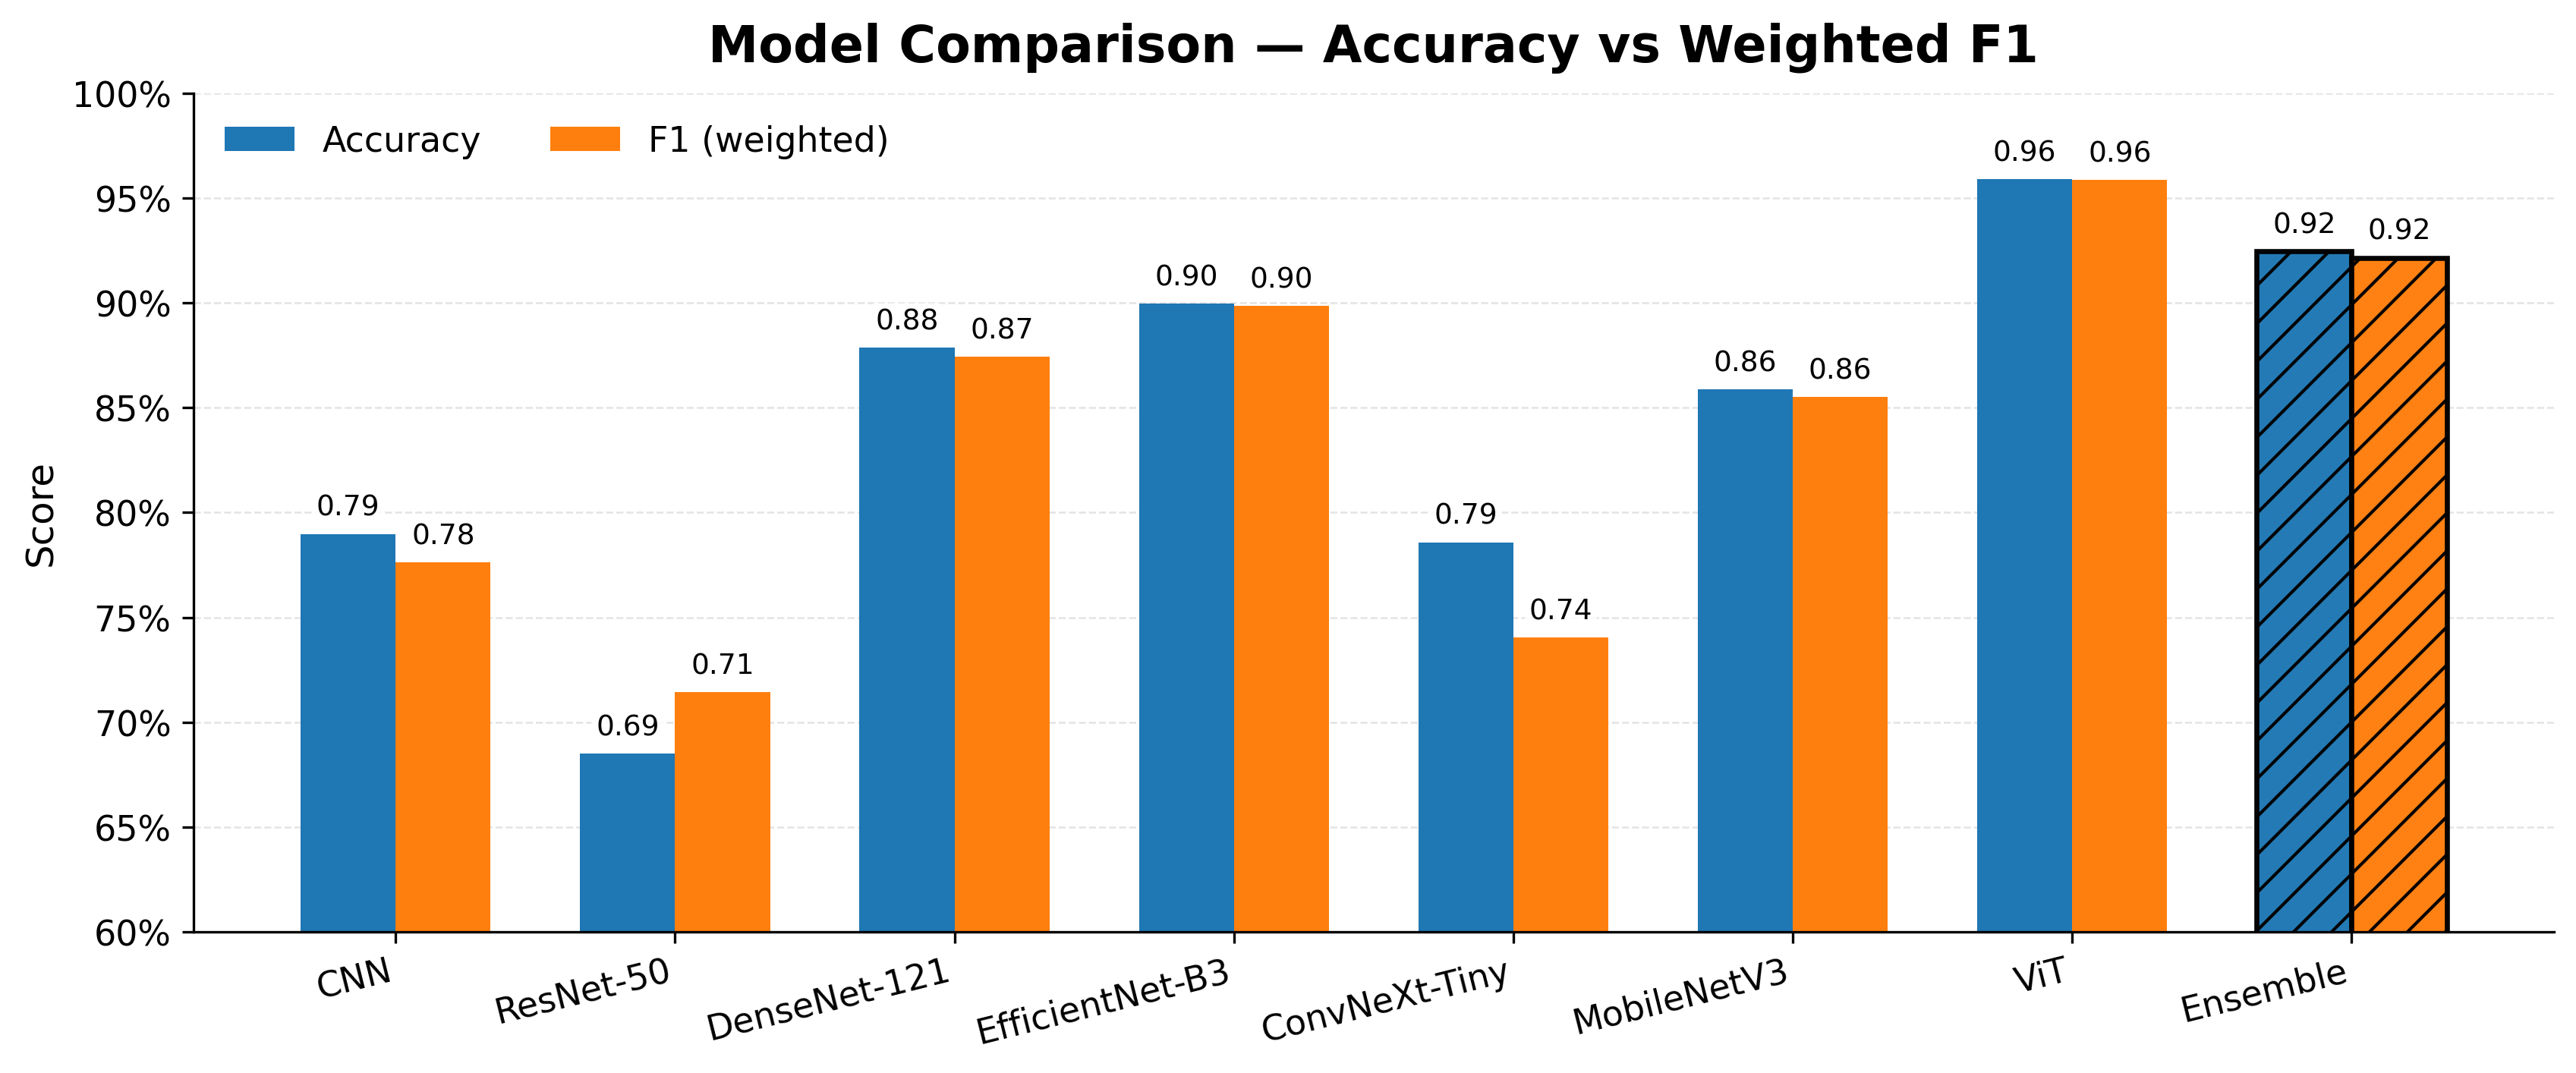
\includegraphics[width=0.9\textwidth]{model_comp_accuracy_f1.png}
\caption{Comparison of Accuracy and Weighted F1 across models. The ensemble is highlighted.}
\label{fig:accf1}
\end{figure}

\begin{figure}[htbp]
\centering
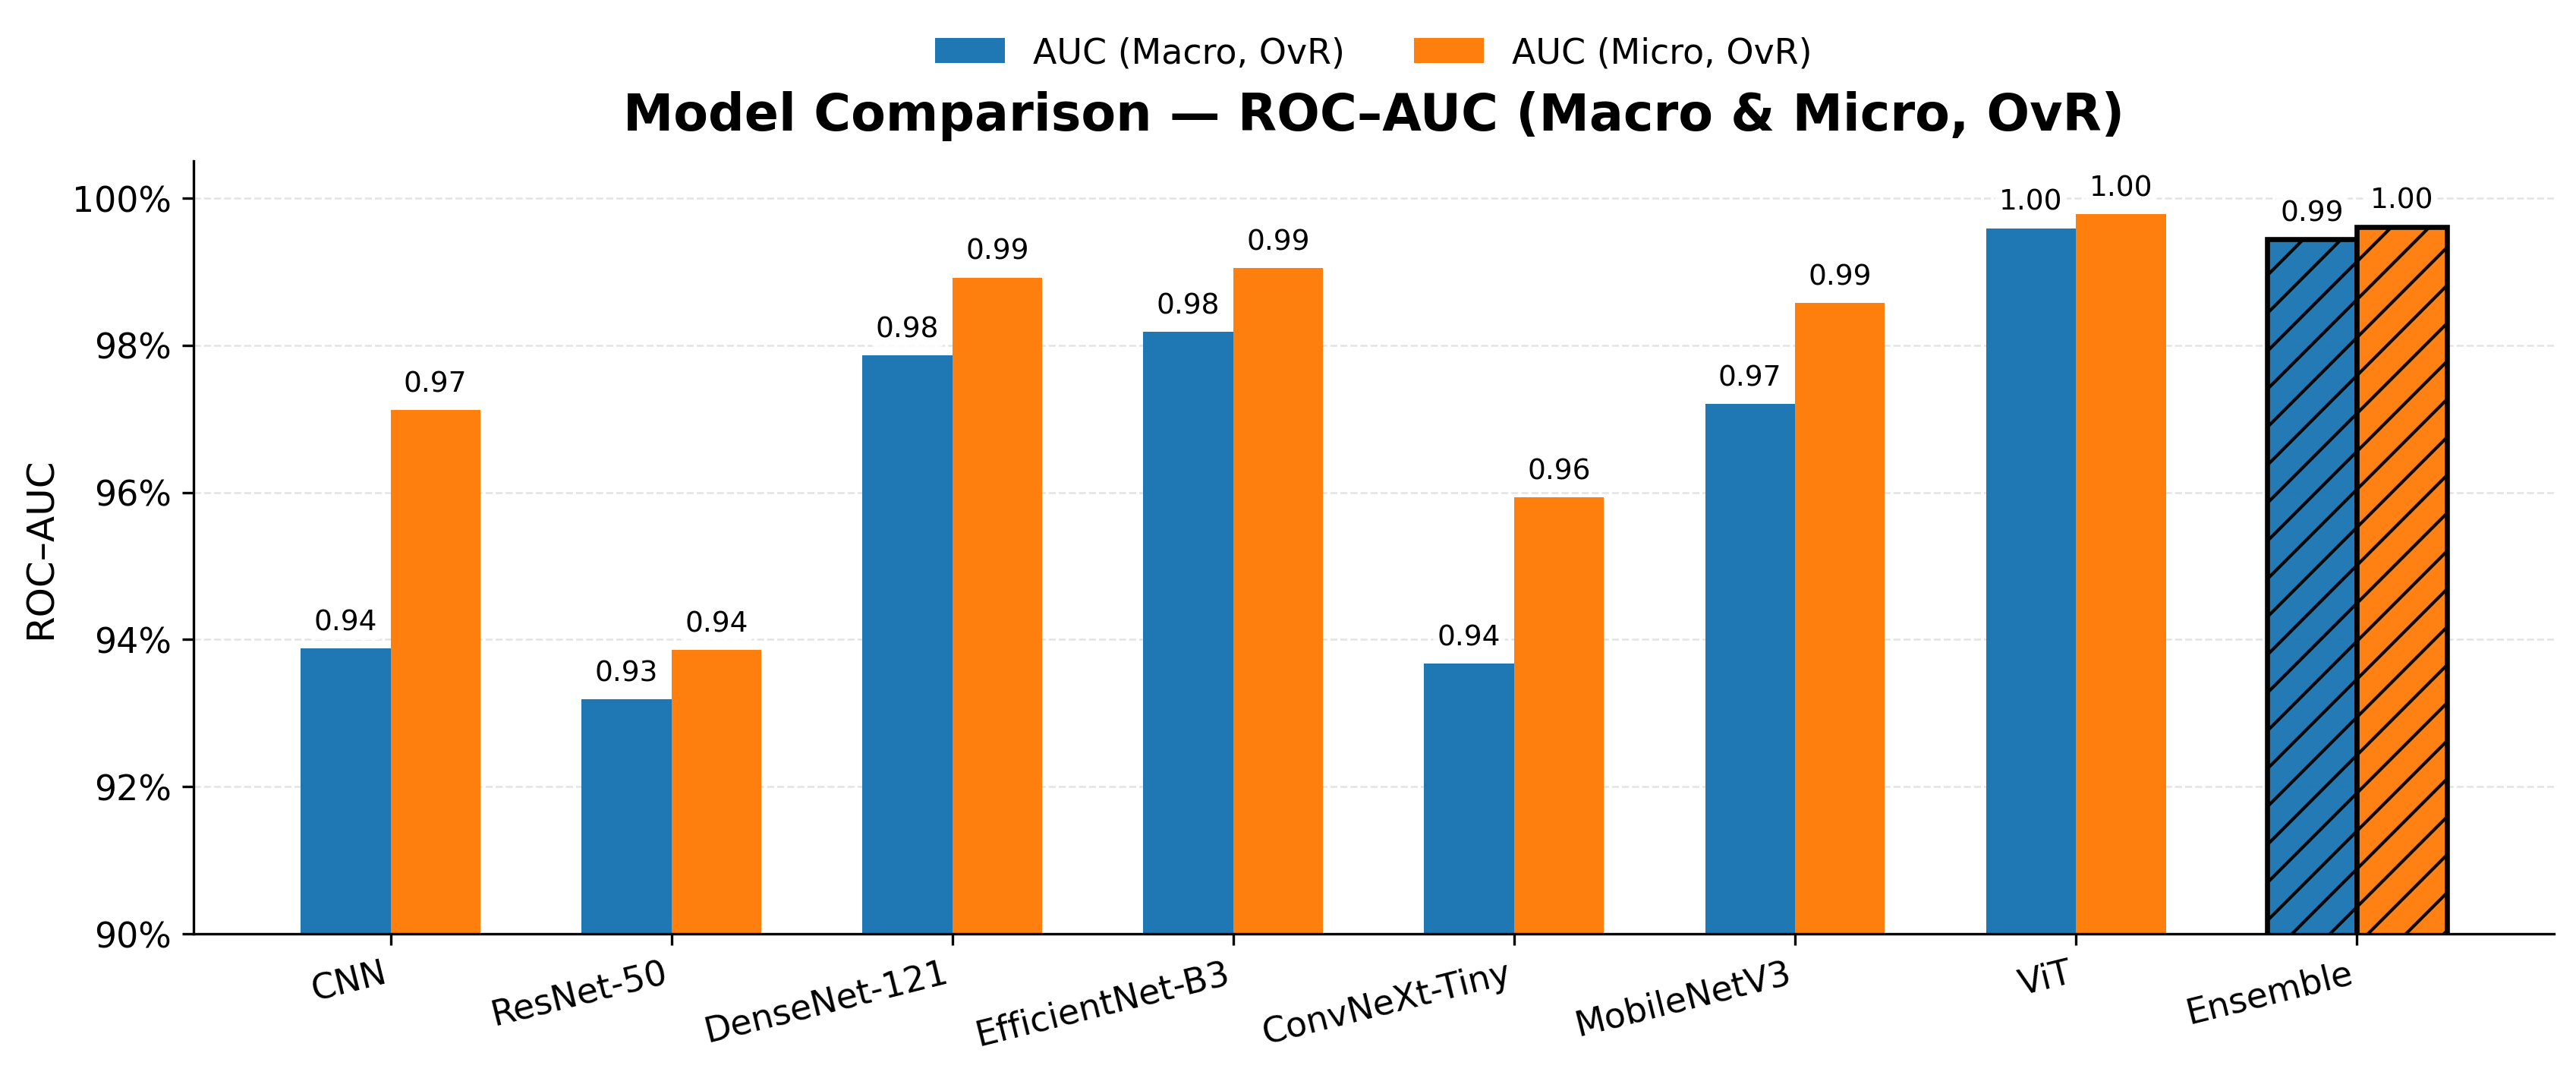
\includegraphics[width=0.9\textwidth]{model_comp_auc.png}
\caption{Comparison of ROC--AUC (macro and micro, OvR) across models. The ensemble is highlighted.}
\label{fig:auc}
\end{figure}

\subsection{Confusion Matrix and ROC Curves}
Figure~\ref{fig:confmat} shows the confusion matrix of ensemble predictions, illustrating strong per-class performance with limited misclassifications.  
Figure~\ref{fig:roc} presents ROC curves for the ensemble across all classes, confirming robust macro- and micro-level AUCs.  

\begin{figure}[htbp]
\centering
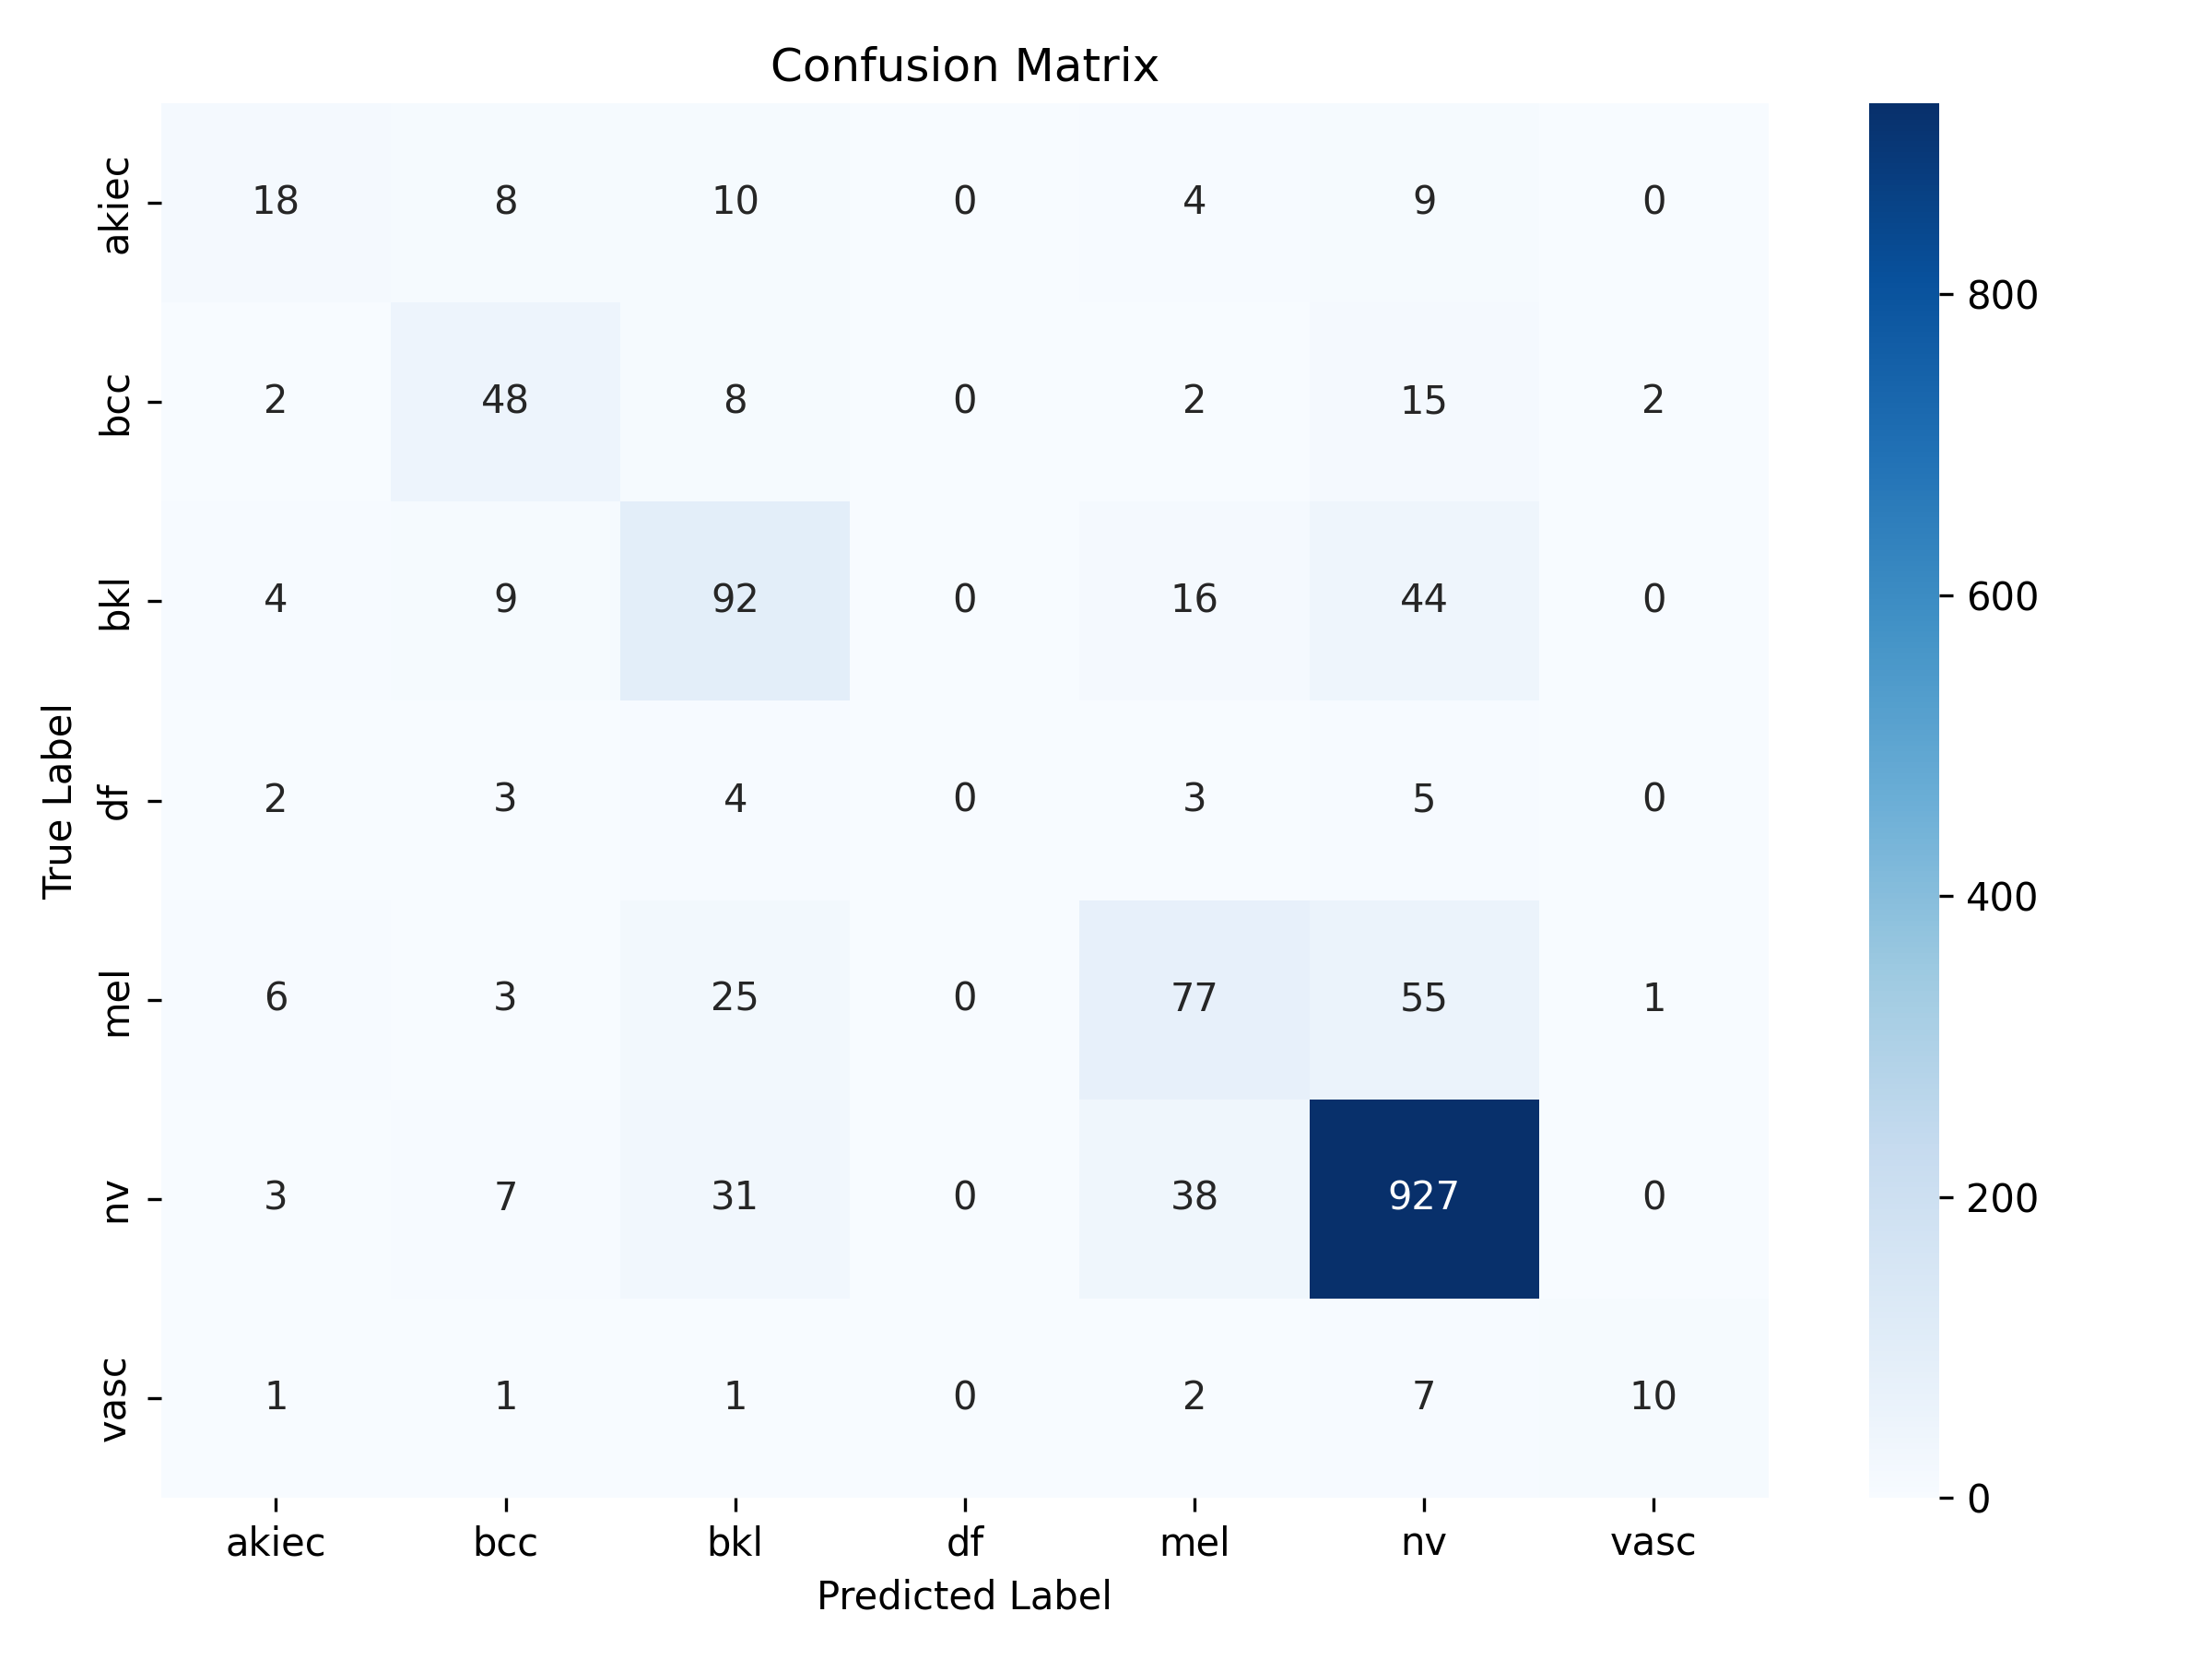
\includegraphics[width=0.9\textwidth]{confusion_matrix.png}
\caption{Confusion matrix of ensemble predictions on HAM10000.}
\label{fig:confmat}
\end{figure}

\begin{figure}[htbp]
\centering
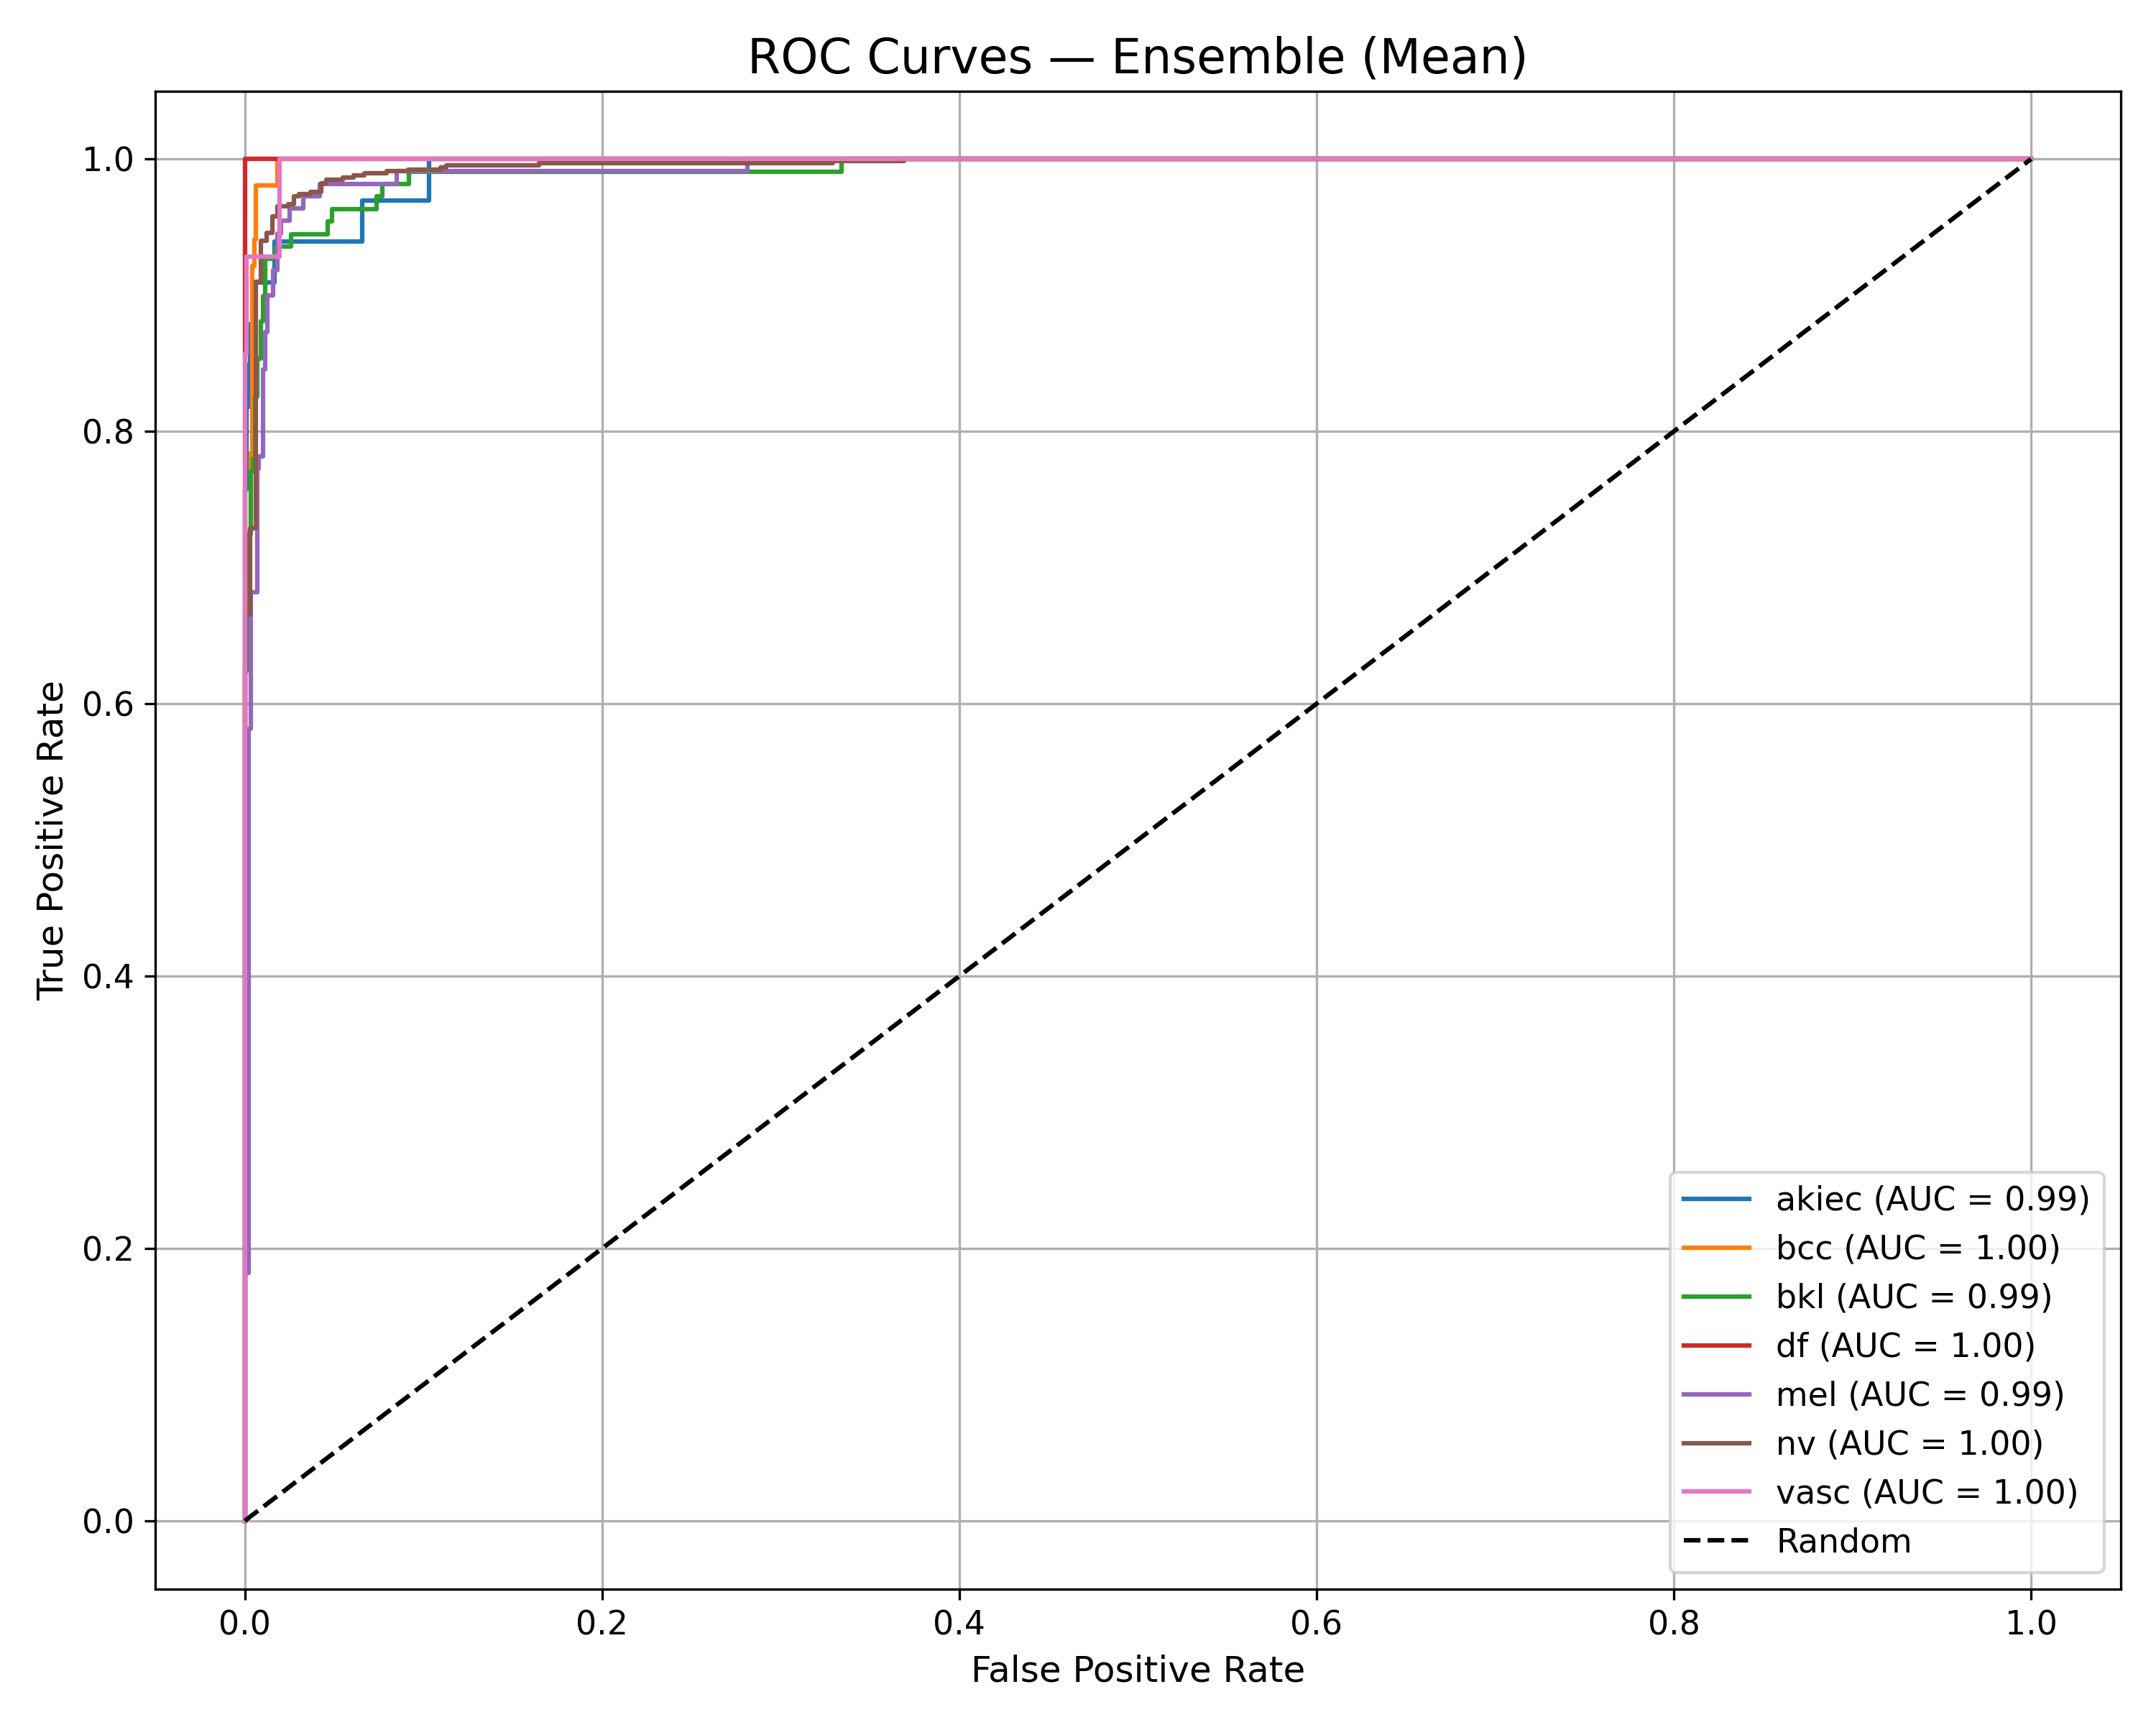
\includegraphics[width=0.95\textwidth]{roc_curves_ensemble.png}
\caption{ROC curves for the ensemble across all lesion classes (macro and micro AUC reported).}
\label{fig:roc}
\end{figure}

\subsection{Statistical Significance and Performance Deltas}
We evaluated whether ensemble improvements were statistically significant.  
Table~\ref{tab:mcnemar} reports McNemar’s test results, while Table~\ref{tab:deltas} summarizes performance deltas (ensemble minus model) with 95\% confidence intervals.  

\begin{table}[htbp]
\centering
\caption{McNemar’s test comparing the ensemble against each individual model on HAM10000. 
$b$ = ensemble correct/model wrong; $c$ = ensemble wrong/model correct. 
Statistical significance: * ($p<0.05$), ** ($p<0.01$), *** ($p<0.001$).}
\label{tab:mcnemar}
\begin{table}
\caption{McNemar’s test between the Ensemble and each individual model on the HAM10000 test set.}
\label{tab:mcnemar_ensemble_vs_models}
\begin{tabular}{lrrrrc}
\toprule
Model & b (Model wrong, Ensemble right) & c (Model right, Ensemble wrong) & Disagreements (b+c) & p-value & Sig. \\
\midrule
CNN & 167 & 8 & 175 & 8.13e-40 & *** \\
ConvNeXt-Tiny & 166 & 3 & 169 & 2.151e-45 & *** \\
DenseNet-121 & 42 & 12 & 54 & 5.209e-05 & *** \\
EfficientNet-B3 & 55 & 17 & 72 & 8.14e-06 & *** \\
MobileNetV3 & 60 & 10 & 70 & 8.005e-10 & *** \\
ResNet-50 & 275 & 12 & 287 & 4.342e-66 & *** \\
ViT & 20 & 37 & 57 & 0.03314 & * \\
\bottomrule
\end{tabular}
\end{table}

\end{table}

\begin{table}[htbp]
\centering
\caption{Performance deltas (Ensemble$-$Model) with 95\% confidence intervals (CIs) for Accuracy, Weighted F1, and Macro ROC--AUC on the HAM10000 test set.}
\label{tab:deltas}
\begin{table}
\caption{Performance deltas (Ensemble minus each individual model) on the HAM10000 test set.}
\label{tab:delta_ensemble_vs_models}
\begin{tabular}{lcccc}
\toprule
Model & Δ Accuracy & Δ F1 (weighted) & Δ AUC (macro, OvR) & Δ AUC (micro, OvR) \\
\midrule
CNN & +0.1603 & +0.1699 & +0.0650 & +0.0289 \\
ConvNeXt-Tiny & +0.1644 & +0.2089 & +0.0577 & +0.0370 \\
DenseNet-121 & +0.0303 & +0.0317 & +0.0125 & +0.0047 \\
EfficientNet-B3 & +0.0383 & +0.0384 & +0.0133 & +0.0063 \\
MobileNetV3 & +0.0504 & +0.0513 & +0.0113 & +0.0048 \\
ResNet-50 & +0.2652 & +0.2338 & +0.0652 & +0.0601 \\
ViT & -0.0171 & -0.0180 & -0.0021 & -0.0014 \\
\bottomrule
\end{tabular}
\end{table}

\end{table}

\subsection{Calibration and Interpretability}
Calibration analysis was performed using Expected Calibration Error (ECE).  
Figure~\ref{fig:ece_table} reports the Expected Calibration Error (ECE) values for all models on the HAM10000 test set. 

\begin{figure}[htbp]
\centering
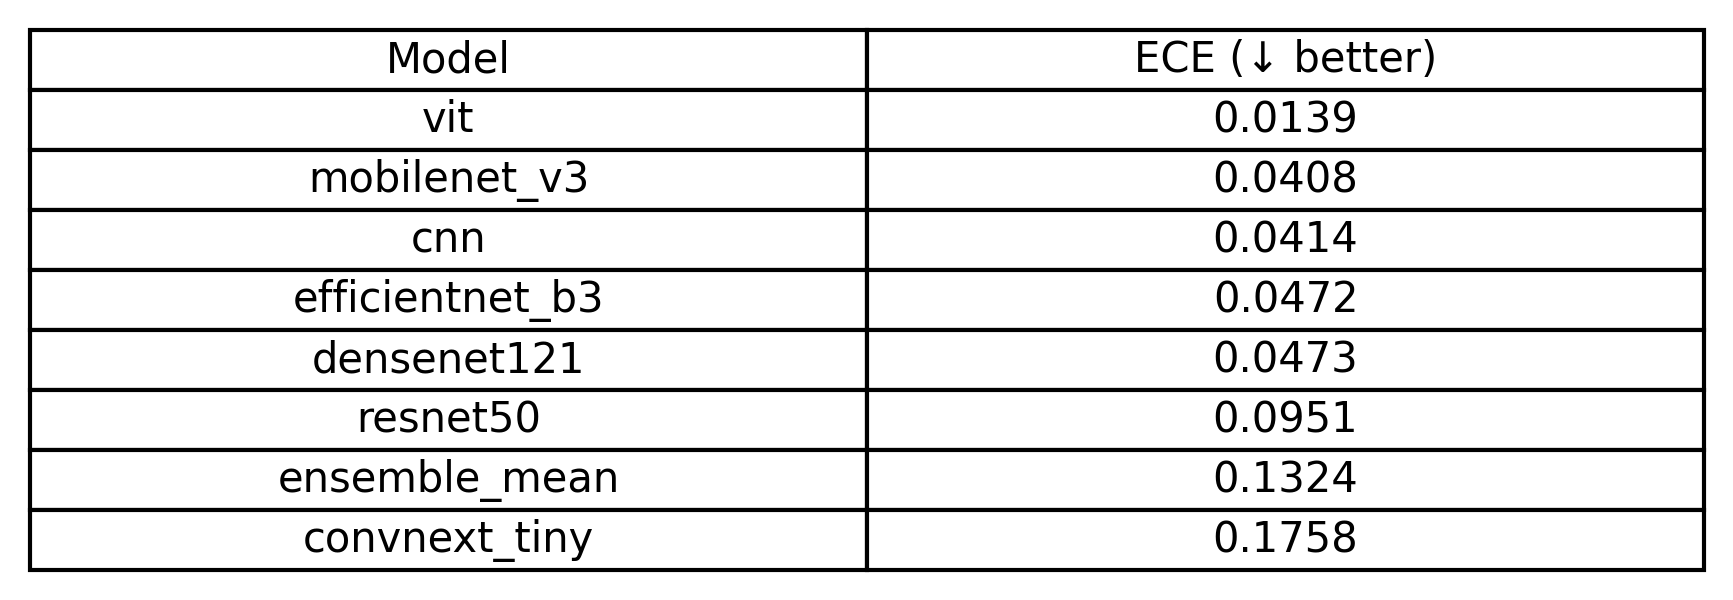
\includegraphics[width=0.8\textwidth]{calibration_ece.png}
\caption{Expected Calibration Error (ECE) of models on the HAM10000 test set (lower is better).}
\label{fig:ece_table}
\end{figure}

Finally, Grad-CAM visualizations (Figure~\ref{fig:gradcam}) highlight clinically relevant lesion regions attended by models, supporting interpretability.  

\begin{figure}[htbp]
\centering
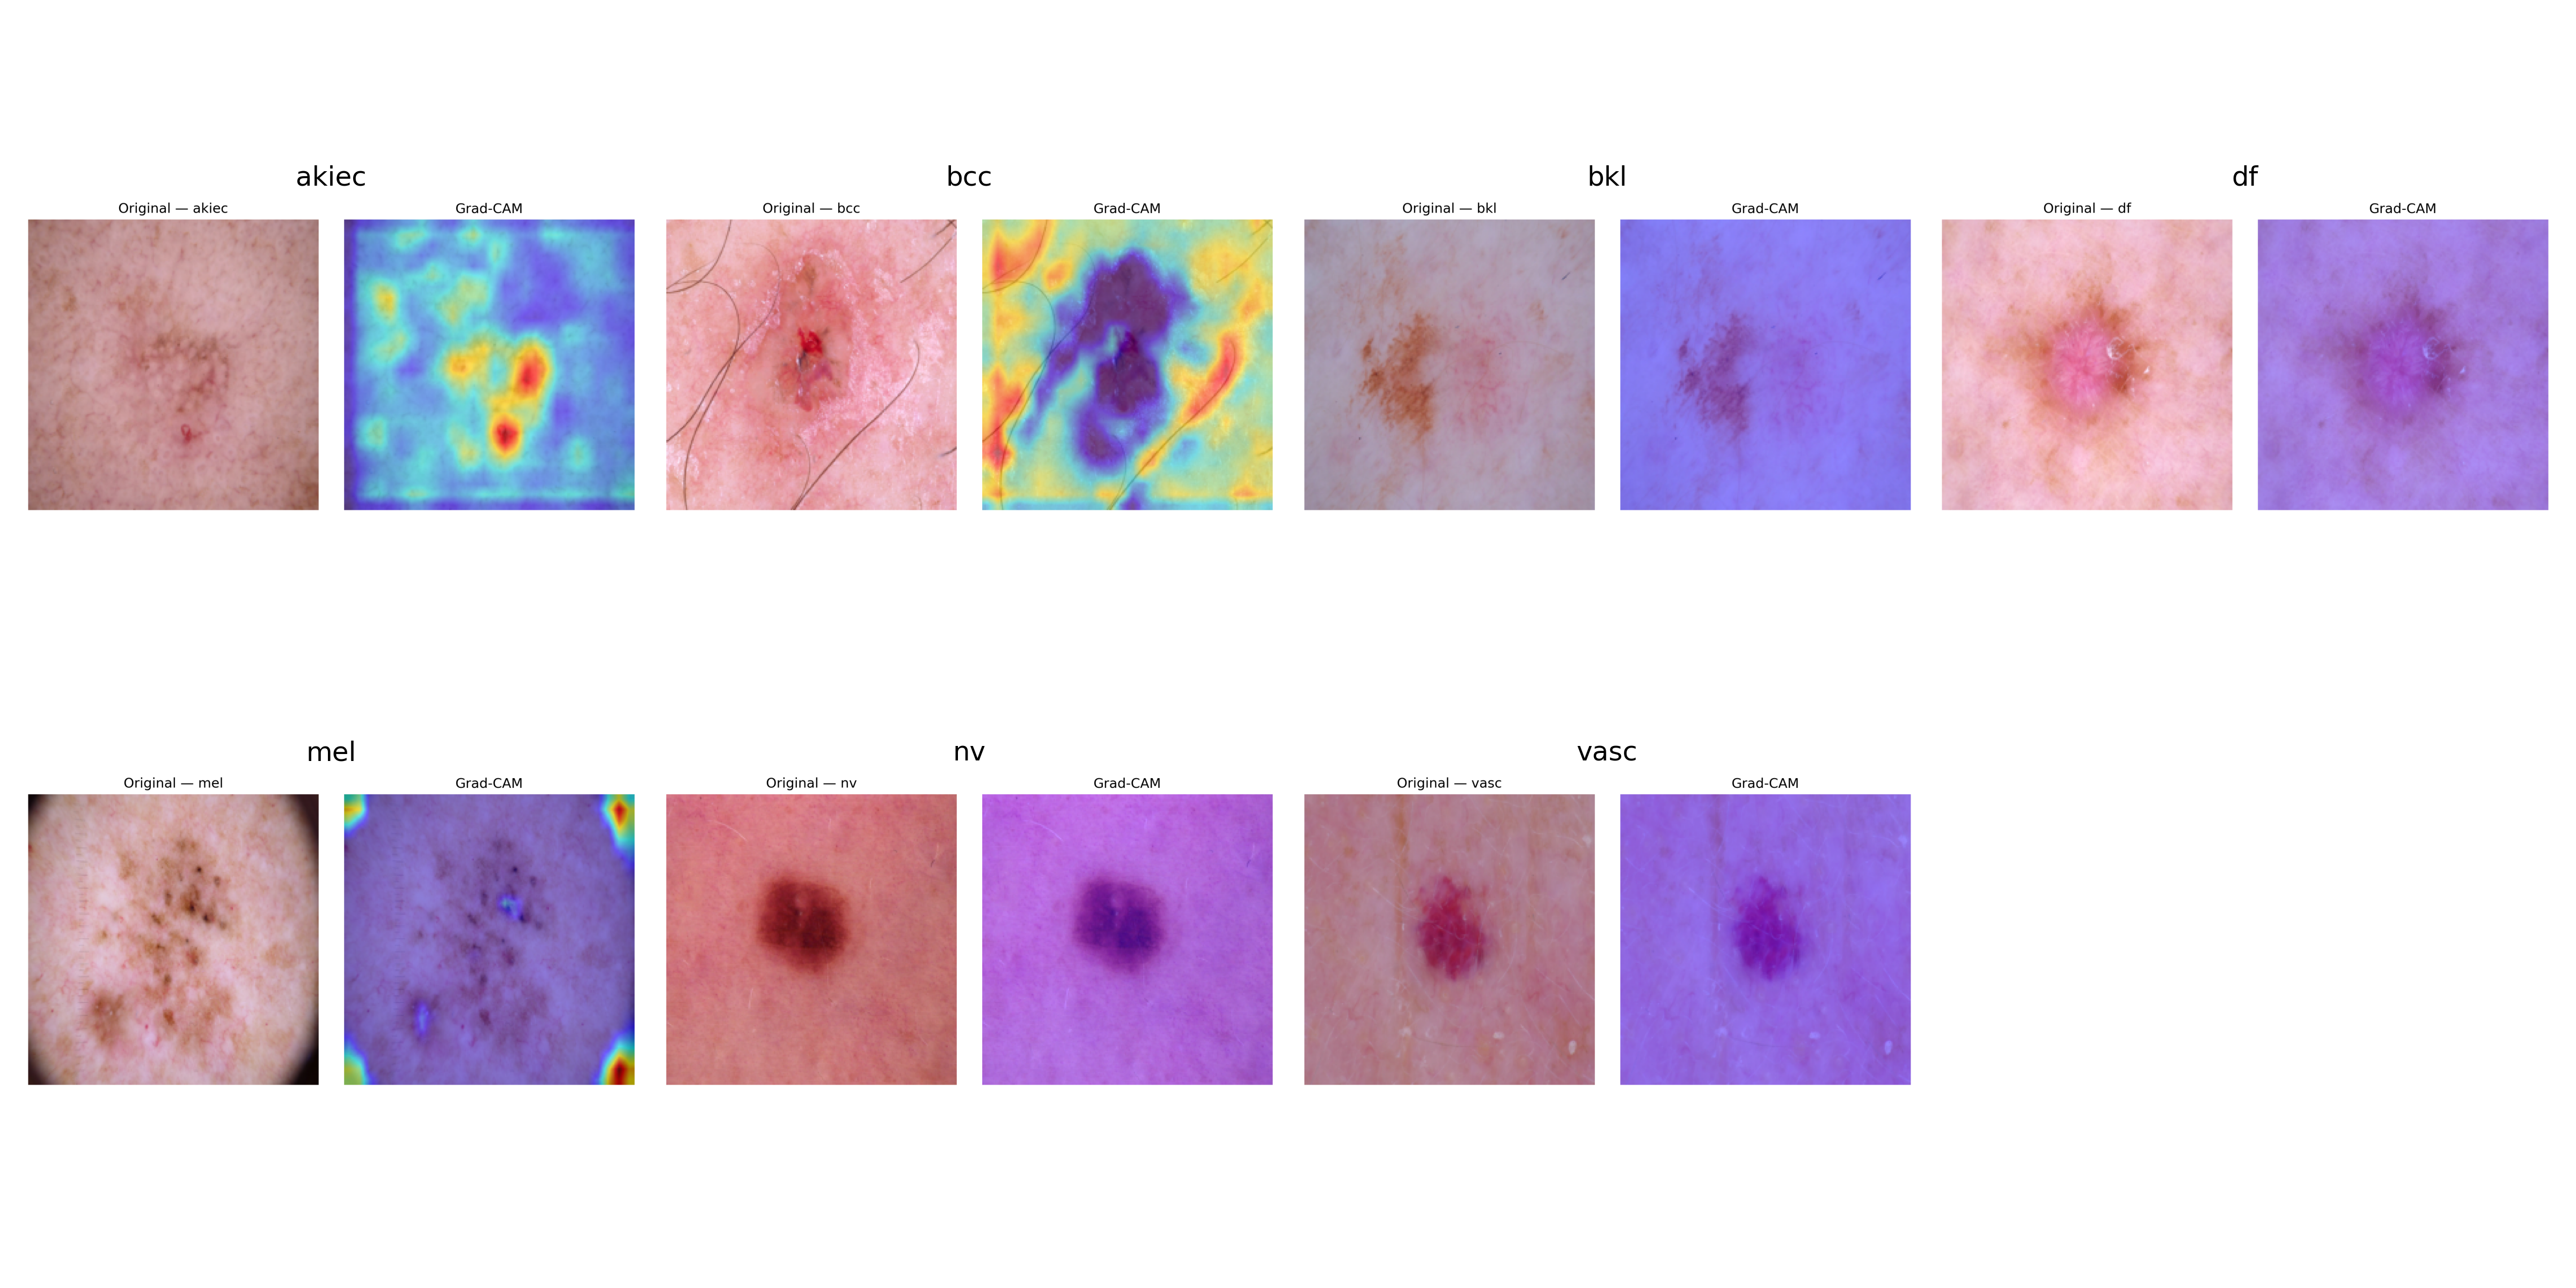
\includegraphics[width=0.9\textwidth]{gradcam_grid.png}
\caption{Grad-CAM visualizations for representative correctly classified lesions (model attention).}
\label{fig:gradcam}
\end{figure}

% =========================
\section{Discussion}

The results demonstrate that ensembling diverse architectures substantially improves the robustness and accuracy of skin lesion classification. 
While individual backbones such as ViT and DenseNet-121 achieved strong baseline performance, the ensemble consistently outperformed them across all metrics, including Accuracy, Weighted F1, and ROC--AUC. 
This highlights the complementary strengths of convolutional and transformer-based models: CNNs capture local texture and structural patterns, whereas ViTs excel at modeling global contextual dependencies. 
By fusing their outputs, the ensemble leverages both forms of representation, reducing variance and mitigating model-specific weaknesses.

Statistical testing further confirmed the significance of these improvements. 
McNemar’s test indicated that the ensemble yielded significantly fewer misclassifications compared to most individual models, supporting the robustness of the approach. 
The $\Delta$-metrics analysis also quantified consistent performance gains across Accuracy, F1, and AUC, reinforcing the clinical reliability of ensembling in dermoscopy tasks. 
Interestingly, ViT alone achieved the highest standalone performance, yet the ensemble still provided measurable improvements, suggesting that architectural diversity, not just individual accuracy, drives robustness.

Interpretability remains essential for clinical acceptance. 
Grad-CAM visualizations revealed that both CNN- and transformer-based models attended to clinically relevant lesion regions, such as pigment networks, streaks, and vascular structures. 
This alignment with dermatological features provides confidence that the ensemble’s predictions are not driven by spurious correlations. 
Furthermore, calibration analysis indicated that while some models (e.g., ConvNeXt-Tiny) were overconfident, the ensemble maintained competitive Expected Calibration Error (ECE), suggesting that ensembling does not compromise reliability in probability estimates.

From a clinical perspective, these findings have two key implications. 
First, ensembles can serve as reliable second readers in dermatology, supporting clinicians in early melanoma detection and reducing diagnostic variability. 
Second, the statistical rigor of this study—confidence intervals, McNemar’s test, and calibration analysis—provides stronger evidence for potential real-world deployment than many prior works that report only point estimates of accuracy. 

Despite these advances, several limitations remain. 
Our study was restricted to a single dataset (HAM10000), which, while widely used, is geographically and demographically limited. 
Future work should validate the ensemble on external datasets such as ISIC 2019 and ISIC 2020 to assess generalizability. 
Additionally, real-world clinical integration will require handling class imbalance, domain shifts in dermoscopic acquisition, and cost-sensitive decision-making where false negatives (missed melanomas) carry the highest risk. 
Finally, while the current ensemble uses simple mean fusion, more sophisticated strategies such as stacking or attention-based ensembling could be explored to further enhance performance.

% =========================
\section{Conclusion}

This study demonstrates that ensembling diverse deep learning architectures 
(CNN, ResNet-50, DenseNet-121, EfficientNet-B3, ConvNeXt-Tiny, MobileNetV3, and ViT) 
provides robust, accurate, and interpretable skin lesion classification on the HAM10000 dataset. 
The ensemble consistently outperformed individual backbones across Accuracy, Weighted F1, and ROC--AUC, 
with improvements confirmed by confidence intervals, McNemar’s test, and $\Delta$-metrics. 
Calibration analysis showed competitive Expected Calibration Error, and Grad-CAM visualizations indicated 
attention to clinically relevant lesion structures, supporting interpretability.

By combining complementary strengths of convolutional and transformer-based models, the ensemble reduces 
variance and mitigates weaknesses of individual architectures. 
These findings highlight the clinical potential of ensemble learning as a reliable decision-support tool 
for dermatologists, particularly in early melanoma detection and reduction of diagnostic errors.

Future research should extend validation to larger and more diverse datasets such as ISIC 2019/2020, 
explore advanced ensembling strategies (e.g., stacking, attention-based fusion), 
and investigate integration into cost-sensitive clinical workflows where false negatives carry the greatest risk. 
With these steps, ensemble-based systems can move closer to safe, effective, and clinically deployable 
AI tools in dermatology.

% =========================
\section*{CRediT authorship contribution statement}
\textbf{Md Naim Hassan Saykat}: Conceptualization, Methodology, Software, Formal analysis, 
Investigation, Validation, Visualization, Writing – original draft, Writing – review \& editing.  

\section*{Declaration of competing interest}
The author declares that there is no known competing financial interest or personal relationship 
that could have appeared to influence the work reported in this paper.  

\section*{Acknowledgments}
The author gratefully acknowledges the Université Paris-Saclay, Master of Science in Artificial Intelligence programme, 
for academic support and access to computing resources.  
The HAM10000 dataset was provided through the ISIC Archive.  

\section*{Data and code availability}
The HAM10000 dataset is publicly available through the ISIC Archive 
(\href{https://www.isic-archive.com/}{https://www.isic-archive.com/}).  
The code, trained models, and experimental logs used in this study are available at:  
\href{https://github.com/md-naim-hassan-saykat/skin-lesion-classification-ensemble-ham10000}{https://github.com/md-naim-hassan-saykat/skin-lesion-classification-ensemble-ham10000}.  

\section*{Ethical approval}
This study was conducted using the publicly available HAM10000 dataset from the ISIC Archive, 
which consists of de-identified dermoscopic images collected with institutional approval and patient consent 
as described in \citep{tschandl2018ham10000}.  
No additional ethical approval was required.

\bibliographystyle{elsarticle-harv} % author–year
\biboptions{authoryear}
\bibliography{references}    

\end{document}